\documentclass{beamer}
\usepackage{tikz}
\usetikzlibrary{arrows.meta, positioning, fit, shadows, backgrounds, calc, shapes.symbols, shapes.callouts, overlay-beamer-styles, decorations.pathmorphing}
\makeatletter
\def\tikzopacityregister{1}
\tikzset{
  opacity/.append code={
    \pgfmathsetmacro\tikzopacityregister{#1*\tikzopacityregister}
  },
  opacity aux/.code={ % this is the original definition of opacity
    \tikz@addoption{\pgfsetstrokeopacity{#1}\pgfsetfillopacity{#1}}
  },
  every shadow/.style={opacity aux=\tikzopacityregister}
}
\makeatother

\tikzset{
  every node/.style={font=\scriptsize},
  panel/.style={
    draw=black, rounded corners=3mm, very thick, fill=white,
    drop shadow, inner xsep=5mm, inner ysep=5mm
  },
  card/.style={
    draw=black, rounded corners=3mm, very thick, fill=blue!8,
    drop shadow, minimum height=8mm,
    text width=30mm, align=left, inner xsep=4mm, inner ysep=2mm,
    text=black
  },
  winborder/.style={draw=green!50!black, line width=1.4pt},
  prop/.style={
    draw=black, rounded corners=4mm, very thick, fill=orange!10,
    drop shadow, minimum width=30mm, minimum height=15mm,
    align=center, inner sep=4mm, text=black
  },
  winner/.style={
    draw=black, rounded corners=4mm, very thick, fill=green!15,
    drop shadow, minimum width=30mm, minimum height=6mm,
    align=center, inner sep=5mm, text=black
  },
  longlist/.style={
    draw=black, rectangle, tape, very thick, align=center, inner sep=4mm,
    tape bend top=none,tape bend height=0.2cm,
    text=black, minimum height=1cm, drop shadow
  },
  arr/.style={-{Stealth[length=3mm,width=2.2mm]}, line width=1.0pt},
  back/.style={arr, dashed},
  garr/.style={-{Stealth[length=3mm,width=2.2mm]}, line width=1.0pt, green!50!black},
}

\title{What online advertising reveals about the limits of standard machine learning theory}
\author{Alex Shtoff}
\institute{TII - Technology Innovation Institute}
\date{July 2026}

\DeclareMathOperator*{\argmax}{argmax}
\DeclareMathOperator*{\argmin}{argmin}
\DeclareMathOperator{\prob}{\mathbb{P}}
\def\vx{\boldsymbol x}
\def\vb{\boldsymbol b}
\def\vv{\boldsymbol v}
\def\vw{\boldsymbol w}

\begin{document}

\frame{
\titlepage
\centering
\begin{tabular}{cc}
     Homepage &  Attendance \\
     \hspace{2em} 
\includegraphics[width=.2\textwidth]{fig/homepage.png}  \hspace{2em} &  \hspace{2em} 
\includegraphics[width=.2\textwidth]{fig/attendance.jpeg} \hspace{2em}
\end{tabular}
}

\begin{frame}
    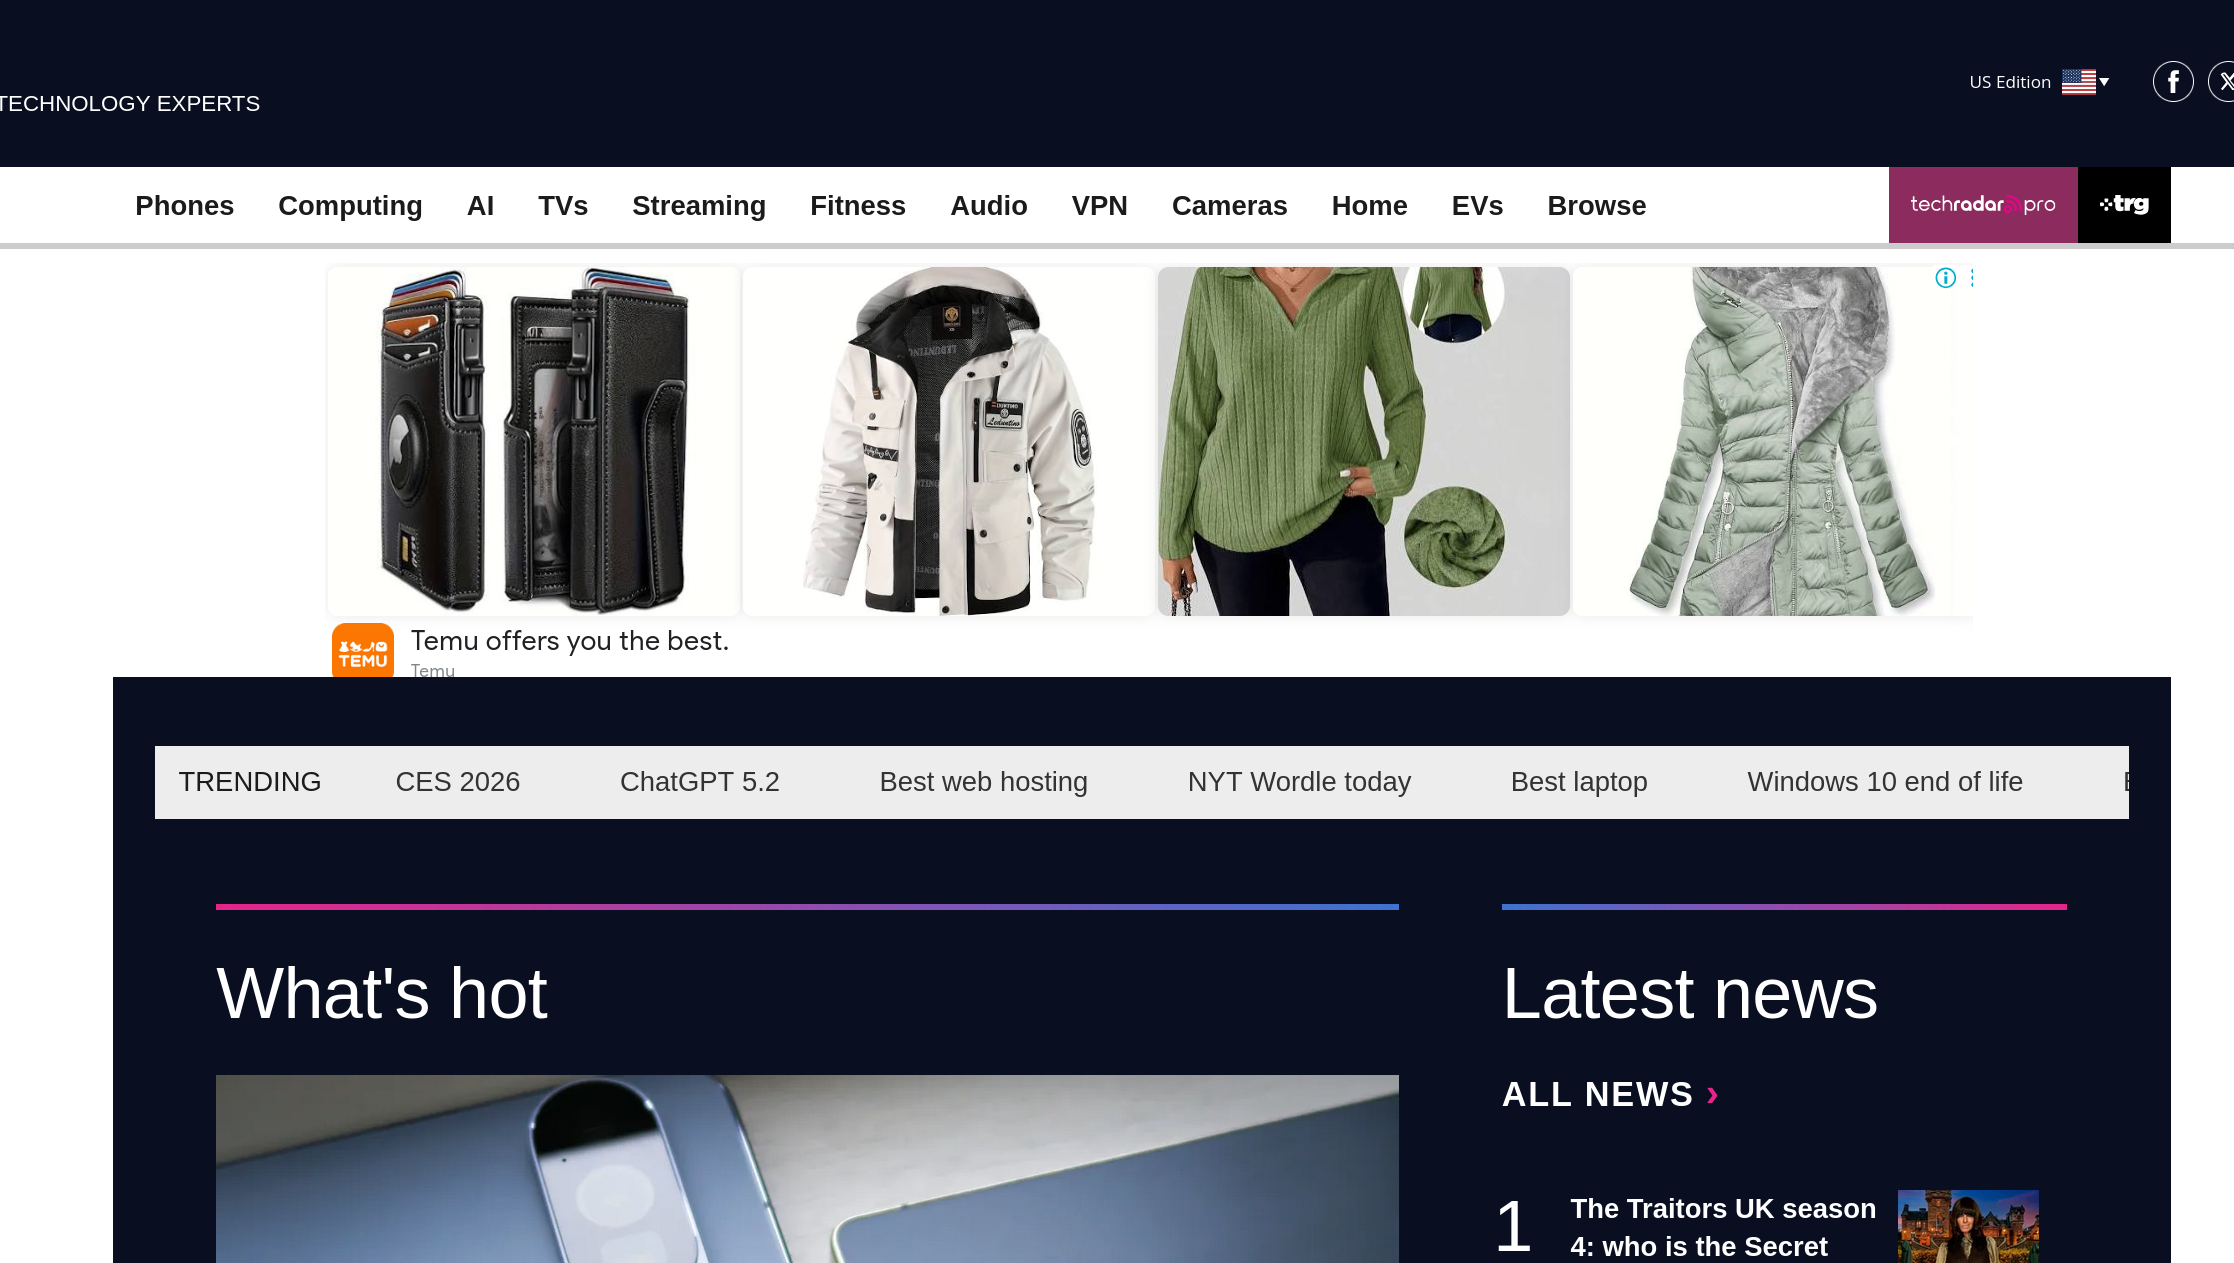
\includegraphics[width=\textwidth]{fig/techradar_ad_example.png}
    \begin{tikzpicture}[overlay, remember picture]
        \draw[red,very thick,dashed,rounded corners] (0.05\textwidth, 0.35\textheight) rectangle (0.95\textwidth, 0.565\textheight);
    \end{tikzpicture}
\end{frame}


\begin{frame}{Standard RecSys flow}
    \centering
    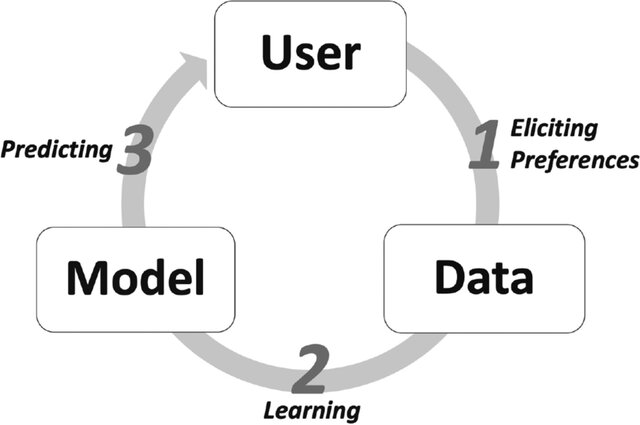
\includegraphics[width=.8\textwidth]{fig/recsys_flow.jpg}
\end{frame}

\begin{frame}{Model training}
    \begin{block}{Train}
        Sample $x_1, \ldots, x_N \sim \mathcal{D}$.
        \[
            \hat{\theta} \in \operatorname*{argmin}_{\theta} \hat{R}(\theta) = \frac{1}{N} \sum_{i=1}^n \ell(x_i; \theta)
        \]
    \end{block}
    \begin{block}{Generalization}
        \[
            R(\theta) = \operatorname*{\mathbb{E}}_{x \sim \mathcal{D}} \sum_{i=1}^n \ell(x; \hat{\theta})
        \]
    \end{block}
\end{frame}

\begin{frame}[t]{Convergence analysis}
    Assume model parameters $\theta \in \mathbb{R}^{\color{blue}d}$. \\
    Training proceeds in iterations (epochs / mini-baches). \\
    After ${\color{red}k}$ training iterations we obtain a trained model $\hat{\theta}$. \\
    \[
        R(\hat{\theta}) - R(\theta^{*}) \leq T({\color{blue}d}, {\color{red}k}).
    \]
\end{frame}

\begin{frame}[t]{Agenda}
    \begin{itemize}
        \item Advertising via bid optimization problem
        \item Why it challenges machine learning theory: train/test setup, convergence analysis, and recsys flow
        \item My personal angle - why ``simple'' models are useful.
    \end{itemize}
\end{frame}

\begin{frame}
\centering
\begin{tikzpicture}
  % Cards
  \node[card] (a1) {\textbf{Shoes}\hfill\textbf{\$2.10}};
  \node[card, below=4mm of a1] (a2) {\textbf{Vacation}\hfill\textbf{\$3.40}};
  \node[card, below=4mm of a2] (a3) {\textbf{Toyota Private}\hfill\textbf{\$1.95}};

  % Candidate panel BEHIND the cards (prevents "empty panel" issue)
  \begin{scope}[on background layer]
    \node[panel, fit=(a1)(a3)] (cand) {};
  \end{scope}

  % Candidate set title
  \node[font=\bfseries\Large, above=3mm of cand.north]  {Candidate set};

  % Highlight winning card
  \draw[winborder, rounded corners=3mm] (a2.north west) rectangle (a2.south east);

  % Property box: top aligned with Shoes (a1)
  \node[prop, anchor=north] (prop)
    at ($(cand.north west)+(-40mm,0)$)
    {\textbf{Property}\\ \texttt{example.com/sports}\\ requests bids};

  % Winner box
  \node[winner, below=6mm of cand.south] (win)
    {\textbf{Winner}\\ Tickets\\ \textbf{\$3.40}};

  % Separated arrows (no overlap)
  \draw[arr] (prop.east)
    to[out=30,in=170,looseness=1.5]
    node[midway,sloped,above] {bid request}
    (cand.north west);

  \draw[back] (win.west)
    to[out=180,in=-90,looseness=1.18]
    node[pos=0.55, below, sloped] {winning ad}
    (prop.south);

  % Max bid arrow
  \draw[garr] (a2.south) -- node[right, xshift=1mm, yshift=-3mm] {max bid} (win.north);
\end{tikzpicture}%
\end{frame}

\begin{frame}
    \centering
    \begin{tikzpicture}
        % nodes
        \node[prop, anchor=north] (prop) {\textbf{Property}\\ \texttt{example.com/sports}};
        \node[prop, below=5mm of prop.south east ,fill=blue!15] (ssp) {\textbf{Supply-Side Platform} \\ (SSP)};
        \draw[arr] (prop.east) to[out=0,in=90] ($(ssp.north)!0.5!(ssp.north east)$);
        \node[rectangle callout, draw=black, thick, inner sep=2mm, align=center, callout absolute pointer={(ssp.north east)}, visible on=<1>] at (7cm, -2cm) {Represents properties \\ -------- \\ $\rhd$ Google Ad Manager \\ $\rhd$ Magnite \\ $\rhd$ Amazon Publisher Service};       

        \node[prop, right=2cm of ssp.east, draw=red, fill=green!15, visible on=<2->] (dsp1) {\textbf{DSP 1}};
        \node[prop, below=0.5cm of dsp1.south, draw=red, fill=green!15, visible on=<2->] (dsp2) {\textbf{DSP 2}};
        \node[below=0.5cm of dsp2.south, visible on=<2->] (dspdots) {...};
        \node[prop, below=0.5cm of dspdots.south, draw=red, fill=green!15, visible on=<2->] (dspn) {\textbf{DSP n}};

        \node[rectangle callout, draw=black, thick, inner sep=2mm, align=center, callout absolute pointer={($(dspn.west)!0.5!(dspn.south west)$)}, visible on=<2>] at (2cm, -6cm) { \textbf{D}emand \textbf{S}ide \textbf{P}latform \\ Represents advertisers \\ -------- \\ $\rhd$ The Trade Desk \\ $\rhd$ Google Display \& Video 360 \\ $\rhd$ Criteo \\ $\rhd$ Yahoo DSP};

        \draw[arr, visible on=<2>] (ssp.east) -- node[midway,above,sloped, visible on=<2>] {bid req.} (dsp1.west);
        \draw[arr, visible on=<2>] (ssp.east) -- node[midway,above,sloped, visible on=<2>] {bid req.} (dsp2.west);
        \draw[arr, visible on=<2>] (ssp.east) -- node[midway,above,sloped, visible on=<2>] {bid req.} (dspn.west);

        \draw[arr, visible on=<3>] (dsp1.west) -- node[midway,above,sloped,visible on=<3>] {Ad 1 (\$2.5)} (ssp.east) ;
        \draw[arr, visible on=<3>] (dsp2.west) -- node[midway,above,sloped, visible on=<3>] {Ad 2 (\$3)} (ssp.east);
        \draw[arr, visible on=<3>]  (dspn.west) -- node[midway,below,sloped, visible on=<3>] {Ad n (\$1.75)}(ssp.east);

        \node<4>[prop, below=5mm of ssp.south, fill=blue!15,align=left] (auction) {\underline{\large{\textbf{Auction}}} \\ Ad n (\$1.75) \\ \textbf{Ad 2 (\$3)} \\ $\vdots$ \\ Ad n (\$1.75)};

        \draw[arr, visible on=<5>] (ssp.west) to[out=180,in=270] node[midway,left,visible on=<5>] {Ad 2 (\$3)} ($(prop.south)!0.5!(prop.south west)$);
    \end{tikzpicture}
\end{frame}

\begin{frame}
    \centering
    \begin{tikzpicture}[remember picture]
        % nodes
        \node[prop, anchor=north] (prop) {\textbf{Property}\\ \texttt{example.com/sports}};
        \node[prop, below=5mm of prop.south east ,fill=blue!15] (ssp) {\textbf{Supply-Side Platform} \\ (SSP)};
        \node[prop, below=5mm of ssp.south east, draw=red, fill=green!15] (dsp) {\textbf{Demand-Side Platform} \\ (DSP)};
        \node[longlist,draw=red,fill=green!15,right=10mm of dsp.east] (ads) {Ad 1 \\ Ad 2 \\ $\vdots$};
        % arrows
        \draw[arr] (prop.east) to[out=0,in=90] ($(ssp.north)!0.5!(ssp.north east)$);
        \draw[arr] (ssp.east) to[out=0,in=90] node[midway,right] {bid request} ($(dsp.north)!0.5!(dsp.north east)$);
        \draw[arr] (dsp.west) to[out=180,in=270] node[midway,left] {bid + ad} ($(ssp.south)!0.5!(ssp.south west)$);        
        \draw[arr] (dsp.east) -- (ads.west);

        \node[dashed, draw=black, fit=(dsp)(ads), inner xsep=2mm, inner ysep=2mm] {};
    \end{tikzpicture}
    
    \pause
    \vfill
    \color{blue}{Objective - in {\color{red}\emph{a few milliseconds}}, select an \textbf{ad} coupled with a \textbf{bid}}
\end{frame}

\begin{frame}[t]{Primary sources of revenue}
\begin{itemize}
    \item \color{purple}{Transaction fees (take rate)}
    \item \color{blue}{Premium services}
    \item \color{blue}{Subscription (annual / quarterly fee)}
\end{itemize}
\vfill
\centering
\pause
Business goal - balance {\color{purple}short term revenue} and {\color{blue}long term satisfaction}.
\end{frame}

\begin{frame}[t]{How are bids chosen?}
    \begin{itemize}
        \item \pause Advertiser sets an \emph{objective}\pause, for example:
        \begin{itemize}
            \item max. exposure
            \item avg cost per purchase
            \item...
        \end{itemize}.
        \item \pause DSP defines a utility $u(b, \vx)$ \emph{aligned with the objective}: 
        \begin{itemize}
            \item $b$ is the bid
            \item $\vx = (\vx_{\mathrm{ad}}, \vx_{\mathrm{ctx}})$ is a vector of ad, and context+user features \\\pause
            $\vx_{\mathrm{ad}}$ ex: product price, product category, ... \\
            $\vx_{\mathrm{ctx}}$ ex: site domain, time of day, user device, user OS, ...
        \end{itemize}
    \end{itemize}
    \vfill\pause
    The optimal bid for a given ad, context, and user:
    \[
    b^*(\vx) =\argmax_b u(b, \vx)
    \]
\end{frame}

\begin{frame}[t]{Utility example - avg cost per purchase}
    \pause
    Objective: pay at most $\alpha = \$10$ for each purchase on average.
    \pause
    
    Assume first-price auction - pay what you bid.
    
    \pause
    \[
    u(b, \mathbf{x}) = \left( \alpha \cdot \mathbb{P}(\mathrm{buy} | \mathbf{x}) - b \right) \pause \cdot \mathbb{P}(\mathrm{win} \vert \mathbf{x}_{\mathrm{ctx}}, b) 
    \]
    \pause
    
    In general,
    \[
    u(b, \mathbf{x}) = \left( V(\mathbf{x}) - b \right) \cdot \mathbb{P}(\mathrm{win} \vert \mathbf{x}_{\mathrm{ctx}}, b) 
    \]
    \pause
    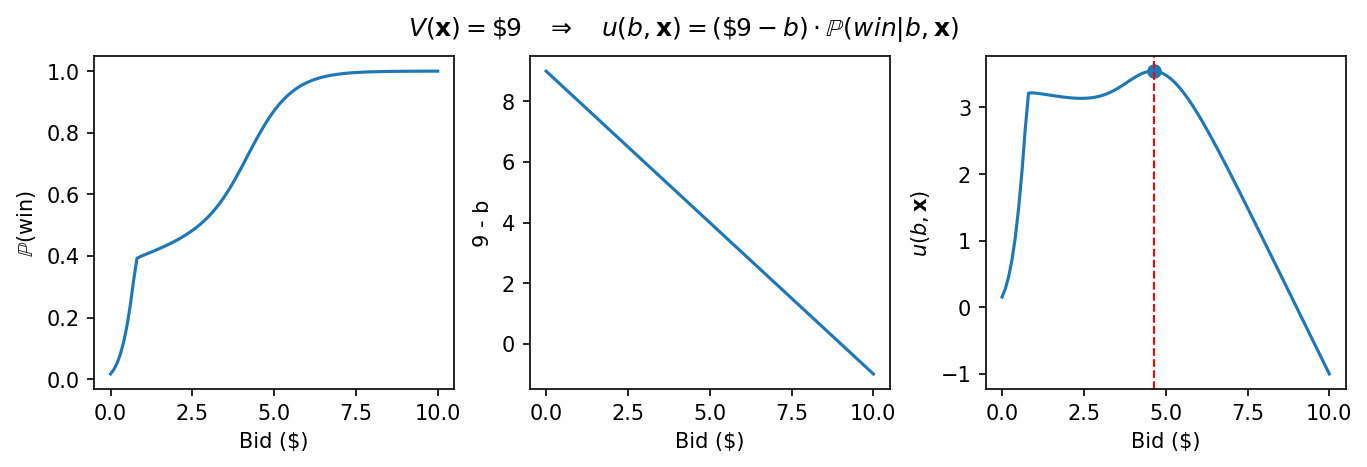
\includegraphics[width=\textwidth]{fig/utility_maximization.png}
    \pause
    \begin{tikzpicture}[overlay]
        \node[%
            cloud callout,
            cloud puffs=15,
            draw=black,
            thick,
            inner sep=-2mm,
            aspect=2.5,
            align=center,
            callout absolute pointer={(8cm, 6.4cm)},
            callout pointer segments=4,
            fill=blue!20,
        ] at (10cm, 5cm) { Machine learned };    
        \pause
        \node[%
            cloud callout,
            cloud puffs=15,
            draw=black,
            thick,
            inner sep=-2mm,
            aspect=2.5,
            align=center,
            callout absolute pointer={(4.3cm, 6.4cm)},
            callout pointer segments=4,
            fill=blue!20,
        ] at (1cm, 4.5cm) { Machine learned };   
    \end{tikzpicture}
\end{frame}

\begin{frame}[t]{DSP ad choice - ideal vs practice}
\begin{tikzpicture}
    \node[longlist,anchor=north,fill=blue!15,minimum width=15mm,inner sep=2mm] (catalogue) {\underline{\textbf{Catalogue}} \\ \\ Ad 1 \\ Ad 2 \\ $\vdots$ };
    \pause
    \node[longlist,fill=blue!15,right=0.75cm of catalogue.east,minimum width=15mm,inner sep=2mm]  (features) {\underline{\textbf{Features}} \\ \\ $\vx_1$ \\ $\vx_2$ \\ $\vdots$ };
    \node[prop,fill=green!15,below=1cm of features.south,align=center,minimum width=15mm] (bidreq) { Bid \\ request};
    \draw[arr] (bidreq.north) -- (features.south);
    \draw[arr] (catalogue.east) -- (features.west);
    \pause
    \node[longlist,fill=blue!15,right=0.75cm of features.east,minimum width=15mm,inner sep=2mm] (optbids) { \underline{\textbf{Optimal bids}} \\ \\ $b^*_1 = \argmax_b u(\vx_1, b)$ \\ $b_2^* = \argmax_b u(\vx_2, b)$ \\ $\vdots$ };
    \draw[arr] (features.east) -- (optbids.west);
    \pause
    \node[longlist,fill=blue!15,right=0.75cm of optbids.east,minimum width=15mm,inner sep=2mm] (optutil) { \underline{\textbf{Utilities}} \\ \\ $u(\vx_1, b_1^*)$ \\ $u(\vx_2, b_2^*)$ \\ $\vdots$};
    \draw[arr] (optbids.east) -- (optutil.west);
\end{tikzpicture}
\pause
\vfill

\centering
\onslide<5->{Highest utility ad(s) is chosen} \\
\onslide<6->{\alert{Now always practical. Phased ranking is typically used.}} \\
\onslide<7->{Example: phase 1 - rank by value, phase 2 - compute bids and rank by utility.}
\end{frame}


\begin{frame}
    \centering
    \Huge
    Before moving forward...
    
    \vspace{5em}
    
    Questions?
\end{frame}


\begin{frame}{Challenge - ranking a huge catalogue in milliseconds}
    \begin{tikzpicture}[
      font=\small,
      box/.style={
        draw=black!60,
        very thick,
        rounded corners=4pt,
        align=center,
        text width=2.75cm,
        minimum height=1.15cm,
        inner xsep=4pt,
        inner ysep=4pt
      },
      rope/.style={
        thick,
        decorate,
        decoration={snake, amplitude=0.45mm, segment length=4.7mm},
        draw=black!65
      },
      pull/.style={
        -{Latex[length=2.5mm]},
        thick,
        draw=black!70
      }
    ]
    
    % Main objects
    \node[box, fill=blue!7] (accuracy) at (-3.55,0)
      {\textbf{Quality}\\ richer model\\ better ranking};
    
    \node[
      circle,
      draw=black!60,
      very thick,
      fill=gray!10,
      align=center,
      minimum size=1.10cm,
      inner sep=1pt
    ] (model) at (0,0)
      {\textbf{model}\\design};
    
    \node[box, fill=orange!10] (speed) at (3.55,0)
      {\textbf{Inference speed}\\ low latency\\ real-time serving};
    
    % Rope
    \draw[rope] (accuracy.east) -- (model.west);
    \draw[rope] (model.east) -- (speed.west);
    
    % Pull arrows
    \draw[pull] (-0.32,0.70) -- (-1.95,0.70);
    \draw[pull] (0.32,0.70) -- (1.95,0.70);
    
    % Pressure labels
    \node[align=center, font=\footnotesize\bfseries] at (-1.85,0.98)
      {quality};
    
    \node[align=center, font=\footnotesize\bfseries] at (1.85,0.98)
      {speed};
    
    \end{tikzpicture}
\end{frame}


\begin{frame}
    \centering
    \emph{Model freshness} is crucial for predictive accuracy
    \vspace{2em}
    {
        \scriptsize
        \begin{thebibliography}{9}
        
            \bibitem{debt}
            D. Sculley, G. Holt, D. Golovin, E. Davydov, T. Phillips,
            D. Ebner, V. Chaudhary, M. Young, J.-F. Crespo, and D. Dennison.
            \newblock Hidden technical debt in machine learning systems.
            \newblock In \emph{Advances in Neural Information Processing Systems},
            vol.~28, pp.~2503--2511, 2015.
            
            \bibitem{trends}
            A. Lommatzsch, B. Kille, and S. Albayrak.
            \newblock Incorporating context and trends in news recommender systems.
            \newblock In \emph{Proceedings of the International Conference on Web Intelligence},
            pp.~1062--1068, 2017.
            
            \bibitem{zhang2020retrain}
            Y. Zhang, F. Feng, C. Wang, X. He, M. Wang, Y. Li, and Y. Zhang.
            \newblock How to retrain recommender system? A sequential meta-learning method.
            \newblock In \emph{Proceedings of the 43rd International ACM SIGIR Conference
            on Research and Development in Information Retrieval},
            pp.~1479--1488, 2020.
        \end{thebibliography}
    }
    \pause
    \vspace{2em}
    {\color{blue}Fast training} is essential for performance
\end{frame}

\begin{frame}
    \begin{tikzpicture}[
      font=\small,
      box/.style={
        draw=black!60,
        very thick,
        rounded corners=4pt,
        align=center,
        text width=2.65cm,
        minimum height=1.05cm,
        inner xsep=4pt,
        inner ysep=4pt
      },
      spring/.style={
        thick,
        decorate,
        decoration={
          coil,
          aspect=0.45,
          amplitude=1.15mm,
          segment length=3.8mm,
          pre length=1.5mm,
          post length=1.5mm
        },
        draw=black!65,
        line cap=round
      }
    ]
        % Main model-design node
        \node[
          circle,
          draw=black!60,
          very thick,
          fill=gray!10,
          align=center,
          minimum size=1.15cm,
          inner sep=1pt
        ] (model) at (0,0)
          {\textbf{model}\\design};
        
        % Objectives
        \node[box, fill=blue!7] (quality) at (-3.55,0)
          {\textbf{Quality}\\ richer model\\ better ranking};
        
        \node[box, fill=orange!10] (inference) at (3.55,0.82)
          {\textbf{Inference speed}\\ low latency\\ real-time serving};
        
        \node[box, fill=orange!7] (training) at (3.55,-0.82)
          {\textbf{Training speed}\\ fast updates\\ fresh model};
        
        % Springs
        \draw[spring] (quality.east) -- (model.west);
        \draw[spring] (model.30) -- (inference.west);
        \draw[spring] (model.-30) -- (training.west);
    
    \end{tikzpicture} 
    \pause
    
    \vspace{5em}
    \textbf{$\mathbb{P}\mathbf{(win)}$}: tractable surplus maximization \\
    \textbf{More}: training without human supervision, interpretability, ...
\end{frame}

\begin{frame}[t]{Some typical models}
    \pause
    \begin{block}{Factorization machines [Rendle et. al. 2016]}
    \begin{align*}
    \Phi_{\mathrm{FM}}(\vx) 
      &= a + \langle \vw, \vx \rangle + \sum_{i=1}^n \sum_{j=i+1}^n \langle \vv_i, \vv_j \rangle x_i x_j \\
      \onslide<3->{&= a + \langle \vw, \vx \rangle + \frac{1}{2}\Bigl \|\sum_{i=1}^n  x_i \vv_i  \Bigr \|^2 - \frac{1}{2} \sum_{i=1}^n \| x_i \vv_i \|^2}
    \end{align*}
    \centering \pause \pause
    Time linear in the dimension of $\vx$!
    \end{block}
    
    \pause
    \begin{block}{Field-weighted factorization machines [Pan et. al. 2018]}
    \[
    \Phi_{\mathrm{FwFM}}(\vx) = a + \langle \vw, \vx \rangle + \sum_{i=1}^n \sum_{j=1}^n \langle \vv_i, \vv_j \rangle R_{f_i,f_j} x_i x_j
    \]
    \end{block}
    \pause
    \centering
    MANY more (DCN, DCNv2, Deep\&Wide, DeepFM, ...)
\end{frame}

\begin{frame}[t]{Win rate prediction models}\pause
    \begin{center}
    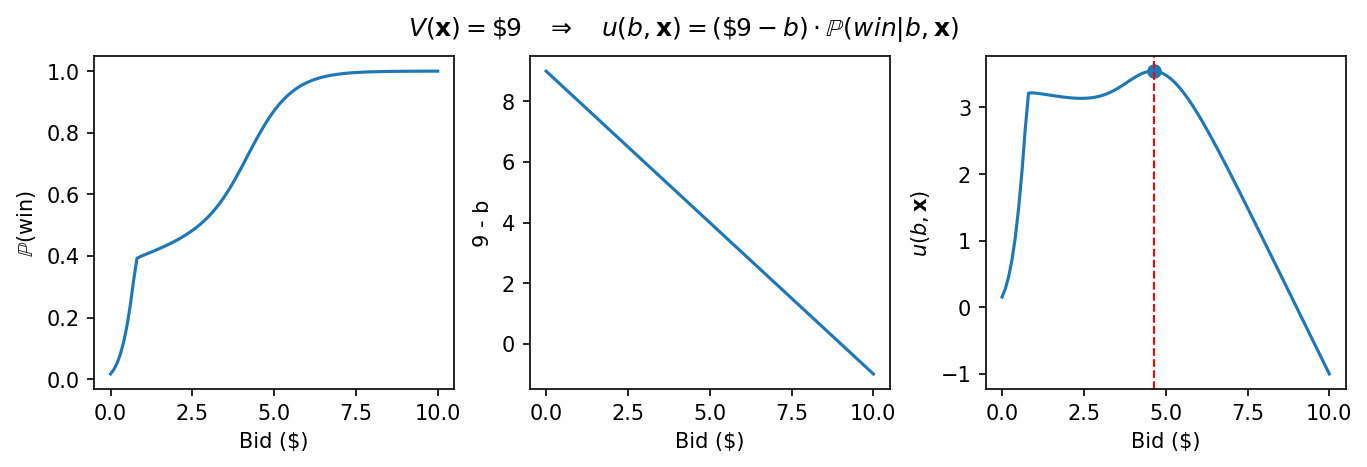
\includegraphics[width=.8\textwidth]{fig/utility_maximization.png}        
    \end{center}
    $\mathbb{P}(\mathrm{win}| \vx, b)$ HAS to be a fast-to-compute function of $b$!
\end{frame}

\begin{frame}[t]
    Bid Shading by Win-Rate Estimation and Surplus Maximization (2020, Pan et. al.):
    \[
        \mathbb{P}(\mathrm{win}| \vx, b) = \sigma(\Phi(\vx) + c\cdot \ln(b)),
    \]
    where $\sigma(x)$ is the sigmoid. \\
    \pause
    \textbf{Pros}: speed, surplus is \emph{unimodal}; \\
    \textbf{Cons}: limited expressiveness

    \centering
    \pause
    \vfill
    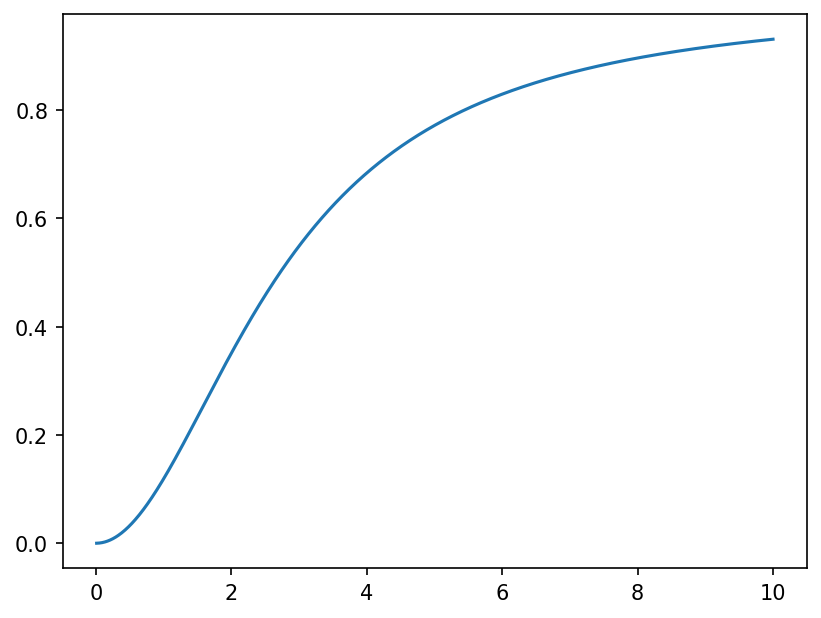
\includegraphics[width=.5\textwidth]{fig/pwins_log_sigmoid.png}
\end{frame}

\begin{frame}[t]
\textit{MEOW: A space-efficient nonparametric bid shading algorithm} (2021, Zhang et. al.) 

\vspace{2em}
Instead of $\sigma(\Phi(\vx) + c\cdot \ln(b))$, learn a table:

\vspace{2em}
\centering
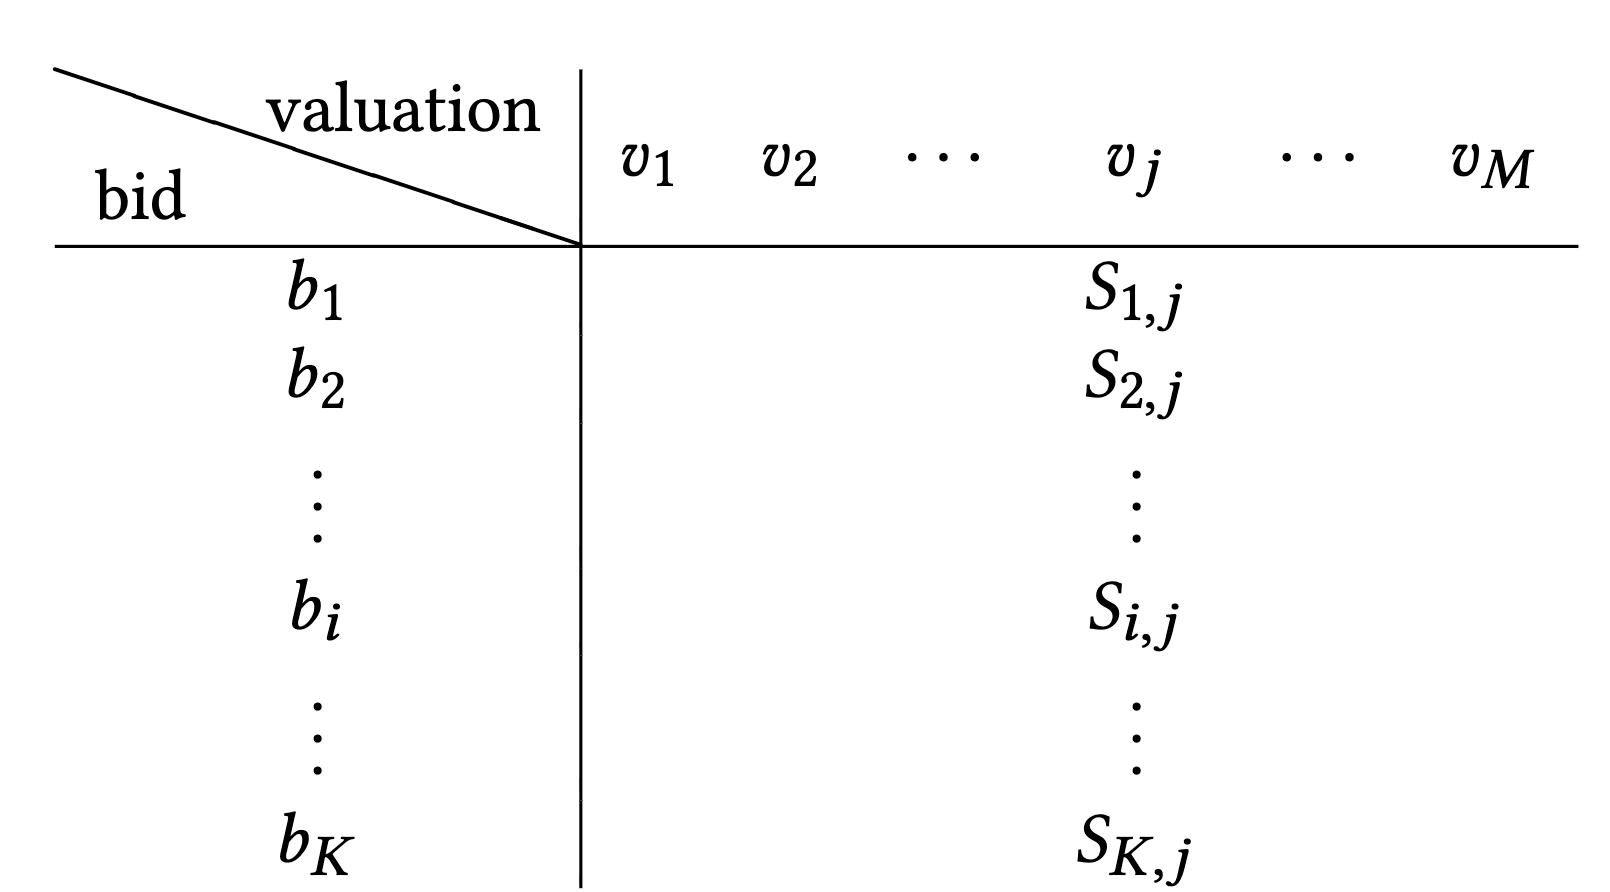
\includegraphics[width=.5\textwidth]{fig/logit_table.png}
\end{frame}

\end{document}
